\documentclass[11pt]{article}
\usepackage[margin=0.85in]{geometry}
\usepackage{fontspec}\setmainfont{Times New Roman}
\usepackage{graphicx,booktabs,array,placeins,microtype,float}
\usepackage[hidelinks]{hyperref}
\usepackage{caption}
\setlength{\emergencystretch}{3em}
\setlength{\parskip}{5pt}
\newcommand{\pep}[2]{#1\textsubscript{#2}}
\title{Computational assessment of EBV-self peptide similarities across HLA class II contexts}
\author{Anish Sharma\textsuperscript{1*}}
\date{September 14, 2026}
\begin{document}
\maketitle
\begin{center}
\small \textsuperscript{1}\textit{Liberal Arts and Science Academy, 1012 Arthur Stiles Road, Austin, TX 78721, USA}\\
\small \textsuperscript{*}Correspondence: \texttt{anishsharma0212@gmail.com}
\end{center}

\begin{abstract}
\textbf{Background} Over the years, researchers have noticed that a prior Epstein-Barr virus (EBV) infection is present in almost all multiple sclerosis patients, with EBV seroconversion being followed by an increase in serological neurofilament light chain, a biomarker indicating neuroaxonal injury. Molecular mimicry between viral and self-antigens is one proposed mechanism for this association.

\textbf{Results} In this study, a multi-stage computational pipeline incorporating NetMHCIIpan, MixMHC2pred, TCR-facing BLOSUM62 similarity scoring, and 3D structural modeling was used to classify candidate EBV-human peptide pairs as candidates for future experimental peptide-HLA binding and register validation. Following an initial rigorous TCR-BLOSUM62 analysis of TCR-contact residues of 6,400 allele-specific pairs across four HLA class II alleles (HLA-DRB1*03:01, *08:01, *13:03, and *15:01), a targeted evidence-review panel of eight pairs underwent further binding affinity and register analysis, yielding two medium-priority pairs and six holds classified as such due to criteria gaps, including predictor discrepancies and register disagreements. In the eight-peptide evidence-review panel, the viral BALF5 (DNA polymerase catalytic subunit) peptide from 627-641 AA paired with the human TALDO1\textsubscript{216-230} (DRB1*15:01) and TALDO1\textsubscript{108-122} (DRB1*13:03) (transaldolase) peptides at rank 14/1600 in *15:01 and rank 13/1600 in *13:03. When the initial screen was expanded to a 49-pair evaluation to address the selectivity concerns, both BALF5-TALDO1 pairs alone were re-recovered, with BALF5\textsubscript{627-641} - TALDO1\textsubscript{216-230} in HLA-DRB1*15:01 being classified by the pipeline as a strong-medium candidate, supported by computational consensus and IEDB-listed BALF5 binding evidence. Structural modeling revealed binding register instability, while several evidence reviews found key gaps in public self-antigen presentation records, especially in alleles outside of the HLA-DR15 system.

\textbf{Conclusions} The study results provide a prioritized shortlist for experimental binding, register-mapping, and T-cell cross-reactivity testing.
\end{abstract}

\section{Background}
Multiple sclerosis (MS) is an autoimmune disease that can cause degeneration of motor, sensory, visual, and cognitive abilities through immune-mediated damage affecting myelin sheaths in the brain, spinal cord, and optic nerves \cite{ninds}. In 2022, Bjornevik et al. studied a cohort of more than 10 million U.S. military personnel, 955 of whom developed MS. Their analysis reported an approximately 32-fold increase in MS risk following EBV infection; cytomegalovirus showed no comparable association. Serum neurofilament light chain increased only after EBV infection, indicating that EBV may precede detectable neurological injury \cite{bjornevik}. Lanz et al. identified an antibody from an MS patient that recognized both EBV EBNA1 and the human CNS protein GlialCAM \cite{lanz}.

Previous studies such as Lanz et al. identified cross-reactive antibodies \cite{lanz}; comprehensive mapping of T-cell cross-reactivity remains incompletely defined. T-cell receptors (TCRs) recognize a peptide presented in the binding groove of a human leukocyte antigen (HLA) molecule rather than the peptide alone. Sequence-only peptide comparisons therefore do not define the HLA-binding component of immune recognition. Different HLA alleles also show distinct structural preferences, affecting pMHC binding affinity and the binding register-the placement of the nine-amino-acid core within the HLA groove. The register determines which residues are anchors and which are potential TCR contacts \cite{brown,sewell}.

The computational pipeline developed here integrates peptide-HLA binding predictions, register-aware sequence alignments, and predicted peptide-HLA structures to prioritize a small subset of viral-self peptide pairs before laboratory testing. Predicted sequence or structural resemblance does not establish stable cell-surface presentation, functional T-cell activation in vivo, or experimentally confirmed registers.

\section{Materials and Methods}
\subsection{Study design}
This study describes a computational prioritization pipeline designed to identify high-interest EBV-human self-peptide candidate pairs for subsequent experimental peptide-HLA binding and binding-register validation. The workflow integrated predicted HLA-binding affinities, register-aware sequence alignments, structural modeling, and downstream evidence review. Computational predictions alone do not establish natural processing and presentation in vivo, surface pMHC stability, or TCR recognition and functional cross-reactivity.

\subsection{Peptide curation and allele-specific pairing}
An EBV repertoire was curated from the Immune Epitope Database (IEDB) by filtering EBV source peptides with positive T-cell assay outcomes from MHC class II alleles in human hosts \cite{iedb}. Human self-proteins included myelin-associated and CNS proteins from positive IEDB MHC-II T-cell records and additional 15-mer peptides derived from UniProt sequences \cite{uniprot}. Duplicate assay records sharing accession, coordinates, and sequence were merged. Imported IEDB records lacking an ``Exact Epitope'' classification or outside 11-30 amino acids were removed, as were sequences containing X, B, or Z. Forty EBV peptides and forty human peptides per allele, selected under evidence and protein-coverage rules, were paired within each allele to create 6,400 allele-specific comparisons.

The initial sequence screen was limited to HLA-DRB1*03:01, HLA-DRB1*08:01, HLA-DRB1*13:03, and HLA-DRB1*15:01. Each HLA allele was evaluated independently; pMHCs from different alleles were not compared. HLA-DRA*01:01 was the alpha chain in every pMHC model.

\subsection{TCR-facing sequence-similarity scoring}
Sequence similarity was calculated with BLOSUM62 \cite{blosum}. Because all non-peptide components are identical within an allele-bound comparison, scoring was restricted to predicted TCR-contact positions P2, P3, P5, P7, and P8 in aligned nine-residue binding cores. Higher scores indicated greater physicochemical resemblance and amino-acid substitution similarity at the potential TCR interface. Scores are relative sequence-prioritization measures, not measures of T-cell recognition, cross-reactivity, presentation, or molecular mimicry. Percentile rankings were calculated independently within each allele's 1,600-pair cohort.

\subsection{Evidence audit and candidate prioritization}
Eight candidate pairs selected from the 6,400-comparison matrix underwent a standardized manual evidence audit. Predicted binding support, predicted register agreement, IEDB sequence and provenance records, public immunopeptidome evidence, viral sequence conservation, and human self-protein tissue expression or rarity were evaluated. Pairs were classified as high priority, medium priority, or hold. No pair was high priority; two were medium priority; and six were held because one or both peptide arms did not meet binding criteria, provenance was unverified, immunopeptidome support was absent, or registers disagreed. The medium-priority pairs were \pep{BALF5}{627-641}-\pep{TALDO1}{108-122} in HLA-DRB1*13:03 and \pep{BALF5}{627-641}-\pep{TALDO1}{216-230} in HLA-DRB1*15:01. The eight-pair audit categories were separate from the later 49-pair provisional classifications.


\subsection{Binding predictions and binding-register analysis}
For the initial eight-pair review, peptide-HLA class II percentile ranks were predicted with NetMHCIIpan-4.3 EL and MixMHC2pred context predictions \cite{netmhc,mix2019}. Full binding consensus required both predictors to return ranks of $\leq5\%$ for both viral and self peptide arms. Lesser binding support required at least one predictor at $\leq5\%$ or both predictors at $\leq20\%$. Peptides were called computationally predicted binders unless IEDB specified exact-match experimental binding-assay records for the matching HLA allele.

Binding-register analysis defined the register as the predicted P1-P9 core within the open-ended HLA class II groove \cite{brown}. NetMHCIIpan-4.3 EL and MixMHC2pred context cores were compared. Any different core sequence, including shifted or overlapping nine-residue windows, was recorded as register disagreement. Major anchor positions (P1, P4, P6, P9) were separated from predicted TCR-facing positions (P2, P3, P5, P7, P8) for downstream analysis.

\subsection{Expanded 49-pair cohort selection}
The expanded 49-pair cohort was analyzed separately from the initial eight-pair evidence audit. All final pair identifiers matched entries in the original 6,400-comparison V3 matrix. The final cohort contained seven HLA-DRB1*03:01 pairs, 14 HLA-DRB1*08:01 pairs, 16 HLA-DRB1*13:03 pairs, and 12 HLA-DRB1*15:01 pairs, corresponding to 98 peptide arms. Thus, the expansion increased candidate coverage while retaining the same four alleles represented in the initial eight-pair audit (Supplementary Methods SM2).

\subsection{Secondary provisional-tier rules}
Secondary provisional tiers were assigned after the expanded 49-pair screen as routing labels for subsequent experimental binding and register-mapping work. No candidate received high-priority status because the automated public-evidence endpoint was unavailable under the frozen review protocol. These provisional labels do not establish peptide-HLA affinity, natural presentation, T-cell recognition, cross-reactivity, molecular mimicry, or disease relevance (Supplementary Methods SM2).

\subsection{pMHC structural modeling}
Heterotrimeric pMHC complexes (HLA-DRA, relevant HLA-DR beta chain, and target peptide) were modeled using the AlphaFold 3 web server, with five returned models per job \cite{af3}. Quality checks verified coordinate completion; peptide pLDDT and peptide-chain ipTM were reported separately because well-defined HLA chains can dominate global complex confidence. The first 85 C$\alpha$ atoms of HLA chain A and chain B were aligned by Kabsch fitting. Peptide backbone RMSD was then measured over an 11-mer window nested around the proposed nine-residue core. AlphaFold outputs were treated as predicted models, not experimental coordinates, and analyzed independently of TCR-docking simulations.

\subsection{Calibration and exploratory modeling}
The literature-derived Hy.2E11 cross-reactive benchmark, \pep{BALF5}{627-641}-\pep{MBP}{85-99}, served as a structural-comparison reference \cite{lang}. The benchmark contains HLA-DRA*01:01-HLA-DRB5*01:01 for BALF5 (PDB: 1H15) and HLA-DRA*01:01-HLA-DRB1*15:01 for MBP (PDB: 1BX2). It was therefore treated as a DR15 haplotype-level control, rather than a same-allele comparison; it does not validate either BALF5-TALDO1 pair or establish biological mimicry.

Poisson-Boltzmann/APBS pMHC surface-potential comparison was explored as an exploratory surface-resemblance descriptor \cite{apbs}. Its score was excluded from primary ranking because a 30-result control gate yielded 15 failed and 12 missing results. Candidate outputs were excluded from ranking and cannot support shared-TCR or cross-reactivity claims; BALF5 replicate models remain exploratory internal predictions rather than docking validation (Supplementary Methods SM8).

\subsection{Statistical calibration and sensitivity analyses}
Statistical methods were implemented to test whether observed TCR-facing BLOSUM62 scores exceeded scores expected after disruption of residue-position alignments. Each HLA allele had its own separate simulation with a starting universe of 40 EBV cores and 40 self cores, making 1,600 pairwise comparisons. Ten thousand simulation replicates were completed independently for each allele at random seed \texttt{20260914} (Supplementary Methods SM3).

Next, binding-threshold sensitivity of the frozen 49-pair panel was evaluated using the predicted binding percentile ranks generated by the IEDB-recommended binding method, NetMHCIIpan 4.3 EL, and MixMHC2pred 2.1 context. The specific percentile thresholds evaluated were 1\%, 2\%, 5\%, 10\%, and 20\% (Supplementary Methods SM3).

Four-metric rank sensitivity was also performed on the four allele-specific cohorts containing 1,600 pairs each. Pairs were evaluated using TCR-facing BLOSUM62, full-core BLOSUM62, TCR-facing sequence identity, and Grantham distance. For a candidate pair to be robust, it needed to be within the top 1\% under at least three metrics, while partially robust pairs did not meet the robust criterion but were within the top 5\% under at least three metrics (Supplementary Methods SM3).

\subsection{Reproducibility}
Reproducibility materials in the project GitHub repository retain software environments, random seeds, input logs, and SHA-256 dataset checksums. Unevaluated or incomplete public-database evidence was labeled ``Not Reported,'' rather than negative. No nominal $p$-values, FDR corrections, or probabilistic ``mimicry probability'' values were used in computational ranking.

\begin{figure}[H]\centering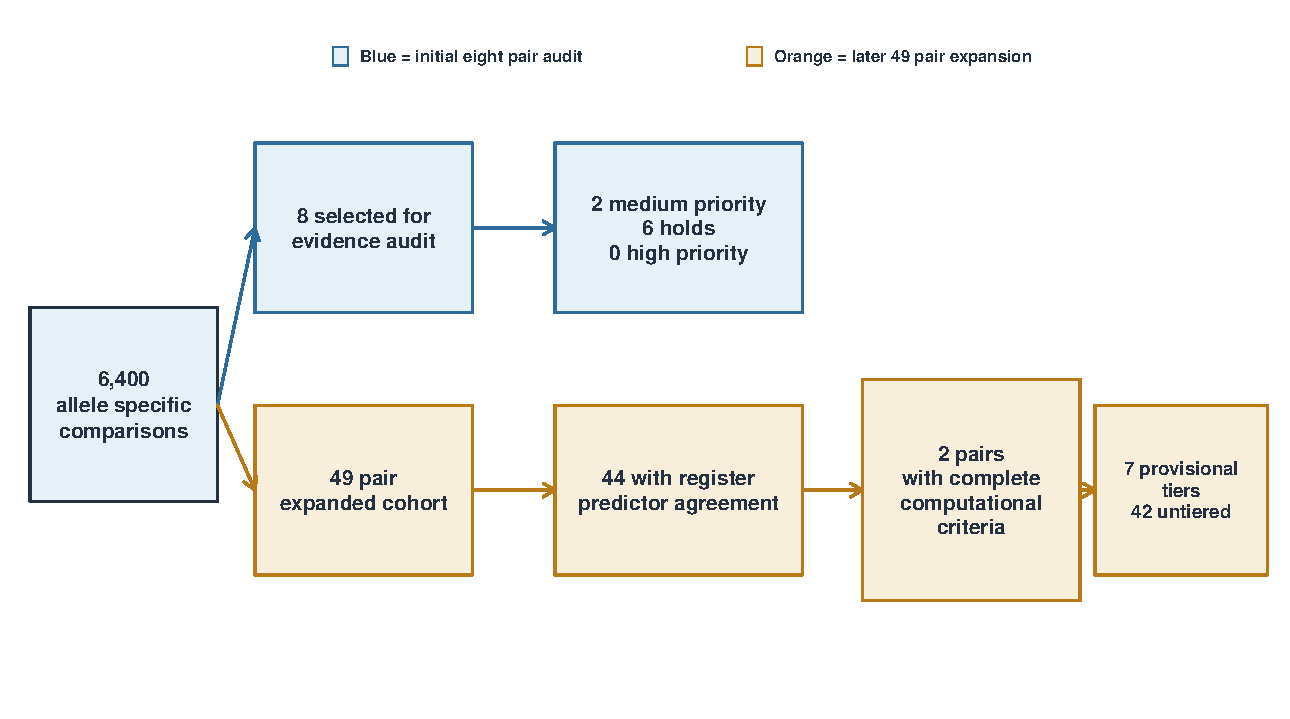
\includegraphics[width=0.95\linewidth]{figures/figure1.pdf}\caption{\textbf{Workflow for computational prioritization of EBV-human peptide pairs.} The 6,400 allele-specific comparisons informed an initial eight-pair evidence audit (blue) and a separate 49-pair expanded cohort (orange). Boxes report the audit or provisional-classification outcomes for each track. The tracks used different review criteria and do not constitute a single sequential funnel.}\end{figure}

\section{Results}
\subsection{Initial sequence comparisons across four HLA alleles}
A total of 6,400 allele-specific peptide-pair comparisons were evaluated across four target alleles, with 1,600 pairs per allele. Sequence-similarity metrics were derived across predicted TCR-contact residues P2, P3, P5, P7, and P8. Score distributions were right-skewed across all alleles, with a small subset of pairs showing elevated TCR-facing sequence similarity (Supplementary Figure S1). These scores represent relative BLOSUM62 substitution-matrix resemblance, not percent identity or a probability of cross-reactivity. The top sequence-ranked pairs within each allele are reported in Supplementary Table S1.

\pep{BALF5}{627-641}-\pep{TALDO1}{108-122} scored 0.28125 in HLA-DRB1*13:03 (rank 13/1,600), while \pep{BALF5}{627-641}-\pep{TALDO1}{216-230} scored 0.31429 in HLA-DRB1*15:01 (rank 14/1,600). These are distinct TALDO1 peptide regions. Both had 40.0\% identity across TCR-contact positions, with full-core identity of approximately 22.2\% in *13:03 and 33.3\% in *15:01.

The four-metric rank sensitivity was calculated for all 6,400 pairs (Figure~\ref{fig:ranksens}). For the DR13 \pep{BALF5}{627-641}-\pep{TALDO1}{108-122} pair, it passed the robustness criteria with a TCR-facing BLOSUM62 rank of 13 (within the top 1\%), TCR-facing identity rank of 2 (within the top 1\%), a full-core BLOSUM62 rank of 173 (outside the top 5\%), and a Grantham distance of 39.2, which is rank 15 (within the top 1\%). For the DR15 \pep{BALF5}{627-641}-\pep{TALDO1}{216-230} pair, it passed the robustness criteria with a TCR-facing BLOSUM62 rank of 14 (within the top 1\%), a full-core BLOSUM62 rank of 3 (within the top 1\%), a TCR-facing identity rank of 4 (within the top 1\%), and a Grantham distance of 44.6, which is rank 33 (within the top 5\%). The pairwise within-allele Spearman correlation $\rho$-values ranged from 0.432 to 0.781, showing moderate-to-strong agreement among related sequence metrics. Based on the ranks, DR13 and DR15 were both determined to be robust under competition-rank handling. Although neither pair ranked uniformly highly across every metric, the DR13 pair was strong in TCR-facing BLOSUM62, identity, and Grantham similarity, while the DR15 pair was strong in both BLOSUM62 formulations and identity. These results remain prioritization results and are not cross-reactivity evidence.

\begin{figure}[H]\centering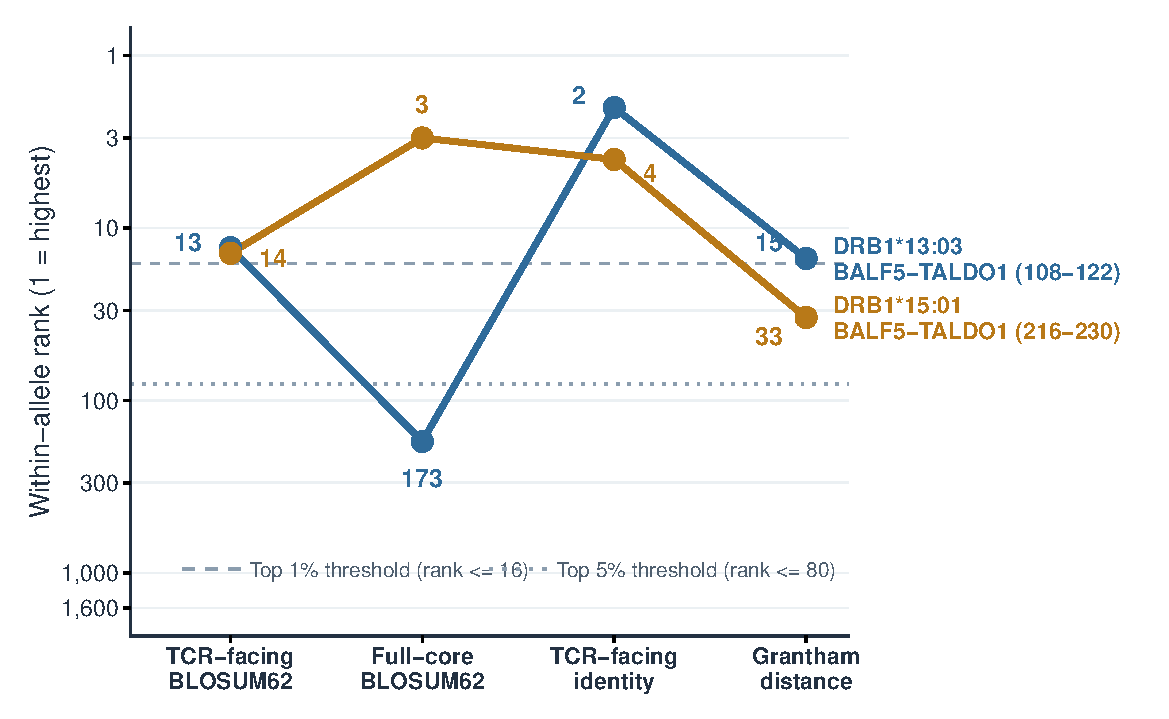
\includegraphics[width=0.90\linewidth]{figures/figure4.pdf}\caption{\textbf{Four-metric rank sensitivity of the BALF5-TALDO1 pairs.} Within-allele competition ranks are shown for TCR-facing BLOSUM62 similarity, full-core BLOSUM62 similarity, TCR-facing sequence identity, and Grantham distance. The vertical axis uses a reverse logarithmic scale, such that rank 1 indicates the greatest similarity. The HLA-DRB1*13:03 and HLA-DRB1*15:01 comparisons contain TALDO1\textsubscript{108-122} and TALDO1\textsubscript{216-230}, respectively.}\label{fig:ranksens}\end{figure}

\subsection{Constrained-null simulation results}
Four of the eight audited pairs had nominal unadjusted $p$ values below 0.05, but none met $q<0.05$ after Benjamini-Hochberg adjustment (BH $q=0.0632$-$0.0819$). Complete pair-specific outputs, including null medians, 95\% null intervals, and maxT $p$ values, are reported in Supplementary Table S4. This process only evaluates sequence-score extremeness and does not provide information about presentation, TCR recognition, or cross-reactivity.

\subsection{Initial Eight-Candidate Evidence Review}
Eight candidates selected from the 6,400-pair matrix underwent deep evidence review, yielding two medium-priority candidates, six holds, and zero high-priority candidates (Supplementary Table S2). The two medium-priority candidates were \pep{BALF5}{627-641}-\pep{TALDO1}{108-122} in HLA-DRB1*13:03 and \pep{BALF5}{627-641}-\pep{TALDO1}{216-230} in HLA-DRB1*15:01. Binding-prediction concordance is shown in Supplementary Figure S2.

Both BALF5-TALDO1 pairs showed predicted core-register agreement, although the registers remain unconfirmed experimentally. Neither pair satisfied full binding consensus. For the HLA-DRB1*13:03 candidate, the viral arm met the $\leq5\%$ criterion while the self arm did not. In HLA-DRB1*15:01, neither arm met full-binding consensus. These thresholds describe the initial review; later predictor outputs differed. No corroborating experimental evidence under the review protocol, including IEDB eluted-ligand records or PRIDE-sourced immunopeptidome records, was identified for either self peptide \cite{pride}. The six held candidates had register discordance, insufficient binding support in one or both arms, or absent public experimental evidence. This review was an initial eight-pair evaluation and remained distinct from the later 49-pair provisional tiers.

\subsection{Focused Structural Assessment of Predicted Binding Registers}
The two medium-priority pairs were structurally assessed alongside a DRB5*01:01 restriction test. Thirteen AlphaFold 3 jobs, each returning five models, generated 65 structural models. All passed checks for coordinate completeness, correct chain identifiers, and peptide-sequence integrity. In HLA-DRB1*13:03, viral parent-nested median RMSD was 0.445~\AA{}; BALF5 showed consistent coordinate recovery, whereas TALDO1\textsubscript{108-122} had lower confidence and positional uncertainty. In HLA-DRB1*15:01, viral and human RMSD values were 1.712~\AA{} and 0.888~\AA{}, respectively; viral BALF5 parent models varied, while the TALDO1\textsubscript{216-230} 11-mer was comparatively consistent. In HLA-DRB5*01:01, viral RMSD was 0.247~\AA{} and longer parent-peptide modeling did not stabilize either competing TALDO1 register.

Models of shorter 11-mers frequently converged to consistent placements, but these placements were rarely retained when parent 15-mers were modeled, producing alternate poses and register shifts (Figure~\ref{fig:length}). Peptide-level pLDDT and peptide-chain ipTM were consequently examined separately from global pMHC metrics; HLA confidence can obscure peptide uncertainty. Sequence-predictor register agreement did not establish atomic-backbone structural confirmation.

\begin{figure}[H]\centering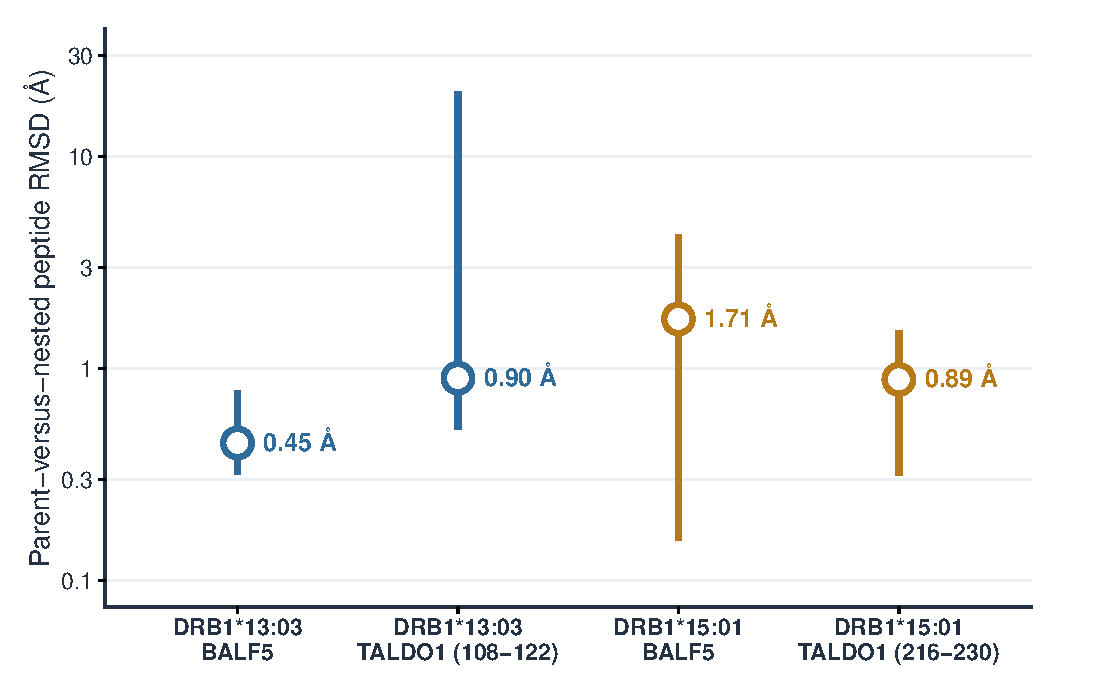
\includegraphics[width=0.90\linewidth]{figures/figure5.pdf}\caption{\textbf{Sensitivity of predicted peptide coordinates to input length.} Parent 15-mer and nested 11-mer models were compared for four peptide arms in HLA-DRB1*13:03 and HLA-DRB1*15:01. Vertical intervals show the minimum-maximum backbone RMSD across the 25 parent-nested model comparisons per arm; open circles show the median. Values describe sensitivity of predicted coordinates to flanking sequence length and do not experimentally establish binding-register placement.}\label{fig:length}\end{figure}
\subsection{Cross-Method Structural Reproducibility}
PANDORA coupled with MODELLER was used for cross-method structural reproducibility \cite{pandora,modeller}. The reciprocal PANDORA controls 1BX2 and 6CQQ were separate from the Hy.2E11 structural reference described above; both passed the pre-defined calibration gate: 120 models were assessed by expected-register recovery, adjacent-decoy comparison, sequence quality control, and template-leakage checks. Each control had at least one top-five model with expected-register core-backbone RMSD below 2~\AA{}, lower top-five median RMSD than adjacent register decoys, and passed exact-sequence and template-leakage tests.

The subsequent ensemble contained 1,200 models spanning BALF5, TALDO1, and eight P6/P7 charge-substitution variants across two structural templates and three register placements (20 models per condition). None of the ten predefined peptides supported the expected NetMHCIIpan/MixMHC2pred register across both templates. A subsequent AlphaFold dataset comprised 150 models from 30 five-model jobs; seven charge-substitution comparisons had uncertain register placement and one was not evaluable because of seed mismatch. Thus, these model outputs did not support interpreting charge substitutions as evidence of disrupted binding.

\subsection{Expanded Assessment of 49 Candidate Pairs}
A separate expanded cohort of 49 pairs was recovered from the 6,400-pair ranking. NetMHCIIpan, MixMHC2pred, and IEDB-recommended binding prediction profiles were completed for 98 peptide arms. Forty-four pairs had at least two predictors selecting the same declared nine-mer core for both arms; this is computational predictor agreement, not experimental register confirmation. Only \pep{BALF5}{627-641}-\pep{TALDO1}{108-122} in HLA-DRB1*13:03 and \pep{BALF5}{627-641}-\pep{TALDO1}{216-230} in HLA-DRB1*15:01 met combined binding and register criteria, with all three predictor ranks $\leq20\%$ for both arms.

For public-evidence assessment, 98 automated IEDB API queries returned zero retrievable records because the endpoint was unavailable. The resulting frozen status was not evaluable, so no candidate could be assigned high priority. Targeted manual IEDB verification later identified an experimentally confirmed binding record for the viral \pep{BALF5}{627-641} peptide in HLA-DRB1*15:01 (IEDB Assay 1774674) \cite{iedb,hansen}. This evidence does not confirm TALDO1\textsubscript{216-230} binding, stable presentation, or dual-reactive T-cell recognition.

\subsection{Secondary Provisional Classifications}
A provisional shortlist contained seven candidates: one strong-medium, two weak-medium, and four strong-low. The remaining 42 candidates were untiered because evidence was insufficient for priority ranking. No pair was high priority because the public-evidence API endpoint was unavailable. These categories are distinct from the earlier eight-pair audit.
The full provisional classification table is reported in Supplementary Table S3.

\section{Discussion}
\subsection{Principal Findings}
This multi-stage computational screening and evidence-review workflow prioritized EBV-human peptide pairs for later experimental validation. Its central findings were two BALF5-TALDO1 pairings, \pep{BALF5}{627-641}-\pep{TALDO1}{216-230} and \pep{BALF5}{627-641}-\pep{TALDO1}{108-122}; despite sharing parent proteins, they are not the same epitope pair. The HLA-DRB1*15:01 pairing had the strongest evidence. The HLA-DRB1*13:03 pairing had weaker support, primarily because allele-specific public presentation evidence was not verified under the review protocol. Secondary candidates included template-consistent \pep{EBNA1}{87-101}-\pep{MBP}{217-233} in HLA-DRB1*15:01 and provisional strong-low candidates such as \pep{EBNA2}{136-150}-\pep{MOG}{97-109} and \pep{EBNA1}{87-101}-\pep{ANO2}{79-93}. The outcome is a computational shortlist for in vitro peptide-HLA binding and register mapping, not a claim of functional molecular mimicry in vivo.

Strong-medium does not mean ``confirmed'' or validated or even ``highest-confidence biological mimic.''

\subsection{Relevance of BALF5-TALDO1}
BALF5-TALDO1 did not have the highest raw sequence-similarity score; EBNA1-ANO2 and EBNA3B-MOG scored higher. Raw sequence alignment was only the first evidence layer. The BALF5-TALDO1 protein pairing was represented by the only two allele-specific pairs in the 49-pair cohort that met combined computational binding and dual-arm register criteria. In HLA-DRB1*15:01, manual recovery of direct binding evidence for viral \pep{BALF5}{627-641} offered limited experimental grounding \cite{iedb,hansen}; the TALDO1 self arm remains unconfirmed by direct-binding or eluted-ligand assays. In HLA-DRB1*13:03, both arms met predictive thresholds, but no allele-specific public binding record was verified under the review protocol. The expanded provisional tiers do not replace the eight-pair audit categories; they derive from a later protocol with different criteria.

\subsection{Contribution of Structural Analyses}
Agreement among sequence-based register predictors did not guarantee stable structural coordinates. Shorter 11-mer inputs often converged in the models analyzed, whereas the same placements were often lost or shifted with the parent 15-mer input. Peptide-local pLDDT and peptide-chain ipTM were therefore more informative than global pMHC metrics, which can obscure peptide uncertainty through high HLA-chain confidence. AlphaFold 3 and PANDORA outputs showed register drift in the modeled BALF5/TALDO1 charge-substitution inputs. These analyses limit register-specific interpretation; they do not identify whether the observed uncertainty is a property of modeling conditions or of peptide biophysics. The retained EBNA1-MBP PANDORA register supports computational geometric plausibility, not native binding.

\subsection{Linkage to Prior Research}
Bjornevik et al. established the epidemiological link between EBV infection and MS, and Lanz et al. reported antibody cross-reactivity between EBNA1 and GlialCAM \cite{bjornevik,lanz}. These mechanisms differ from pMHC class II T-cell recognition; operationally, T-cell cross-reactivity requires one T cell to recognize more than one distinct peptide-MHC ligand \cite{sewell}. Here, claims remain limited to computational candidate prioritization and predicted pMHC similarity. Literature-associated protein pairs, including EBNA1-ANO2 and EBNA1-MBP, emerged in the screen, but shared parent proteins must be distinguished from exact peptide epitopes \cite{thomas}. Literature-informed pairings were not treated as independent computational validation because their disease association contributed to protein selection.

\subsection{Additional Exploratory Methods}
Electrostatic surface-potential comparison was excluded from primary ranking because its control gate did not discriminate the calibration control from background decoys. TCRModel2 calibration produced acceptable models for 1ZGL but incorrect models for 1YMM and 2WBJ under DockQ and CAPRI criteria. These failures prevent candidate-specific TCR-recognition claims; they do not provide biological evidence that cross-reactivity is absent in vivo.

\subsection{Limitations}
The search space was limited to pre-curated viral epitopes, selected myelin/CNS proteins, and four HLA-DRB1 alleles. HLA-DQ and HLA-DP loci were omitted. Rankings shifted under TCR-facing BLOSUM62, full-core BLOSUM62, and Grantham-distance formulations. Predictors may share training data, potentially limiting the independence of their agreement. The unavailable public-evidence endpoint and absent self-peptide records did not establish biological absence of presentation. In silico modeling also cannot account for endogenous antigen processing, HLA-DM-mediated peptide editing, pMHC stability, antigen-presenting-cell context, or downstream TCR-signaling thresholds \cite{denzin}.

\subsection{Experimental Next Steps}
Peptide-HLA binding can be quantified for viral and self peptides against recombinant HLA-DRB1 molecules by fluorescence polarization or surface plasmon resonance. Register mapping may use alanine-scanning mutagenesis and structural methods such as X-ray crystallography or cryo-EM. Matched T cells should be tested against both peptide-HLA complexes for dual functional activation. Endogenous processing can be assessed through peptide elution and mass spectrometry from infected or inflamed antigen-presenting cells.

\section{Conclusions}
The first experimental priority is HLA-DRB1*15:01 \pep{BALF5}{627-641}-\pep{TALDO1}{216-230}, because of its strong-medium classification, its passing of expanded binding-and-register criteria, and exact allele-specific viral-arm IEDB binding evidence \cite{iedb,hansen}. Recombinant peptide-HLA binding should test viral and self arms separately, followed by register mapping because structural analyses did not identify a single stable backbone register. The next candidate is HLA-DRB1*13:03 \pep{BALF5}{627-641}-\pep{TALDO1}{108-122}; both arms passed the expanded computational gate, while absent public evidence was the major factor limiting its tier. The third priority is HLA-DRB1*15:01 \pep{EBNA1}{87-101}-\pep{MBP}{217-233}, whose predicted register persisted across calibrated PANDORA template analysis despite failure of full binding consensus. The strong-low candidates should follow once binding and register outcomes for these top three are available. Natural presentation should then be tested by immunopeptidomics, followed by matched-TCR assays against both pMHC complexes and functional-activation measurements; docking similarity alone is insufficient.
\section{Abbreviations}
AF3: AlphaFold 3; APBS: Adaptive Poisson-Boltzmann Solver; EBV: Epstein-Barr virus; HLA: human leukocyte antigen; IEDB: Immune Epitope Database; MS: multiple sclerosis; pMHC: peptide-major histocompatibility complex; RMSD: root-mean-square deviation; TCR: T-cell receptor.

\section{Declarations}
\subsection{Ethics approval and consent to participate}
Not applicable. This study used public database records and computational analyses and did not involve new research with human participants or animals.

\subsection{Consent for publication}
Not applicable.

\subsection{Availability of data and materials}
The analysis code, input manifests, derived data, and supplementary materials are available in the EBV-MS Project repository, \url{https://github.com/AnishSharma1/EBV-MS_Project}.

\subsection{Competing interests}
The author declares no competing interests.

\subsection{Funding}
No external funding was received for this work.

\subsection{Authors' contributions}
Anish Sharma developed the study, performed all analyses, and wrote the manuscript.

\subsection{Acknowledgements}
The author thanks Dr Brian Pierce for assistance with T-cell receptor modeling, Dr Olaf Stuve for guidance on peptide expansion across HLA alleles, and colleagues at Karolinska Institutet for discussions that informed the binding-register component of this project.

\FloatBarrier
\begin{thebibliography}{99}
\bibitem{bjornevik} Bjornevik K, Cortese M, Healy BC, et al. Longitudinal analysis reveals high prevalence of Epstein-Barr virus associated with multiple sclerosis. \textit{Science}. 2022;375:296-301. \url{https://doi.org/10.1126/science.abj8222}
\bibitem{ninds} National Institute of Neurological Disorders and Stroke. \textit{Multiple Sclerosis: Hope Through Research}. \url{https://www.ninds.nih.gov/health-information/disorders/multiple-sclerosis}
\bibitem{lanz} Lanz TV, Brewer RC, Ho PP, et al. Clonally expanded B cells in multiple sclerosis bind EBV EBNA1 and GlialCAM. \textit{Nature}. 2022;603:321-327. \url{https://doi.org/10.1038/s41586-022-04432-7}
\bibitem{iedb} Vita R, et al. The Immune Epitope Database (IEDB): 2024 update. \textit{Nucleic Acids Research}. 2025;53:D436-D443. \url{https://doi.org/10.1093/nar/gkae1092}
\bibitem{uniprot} The UniProt Consortium. UniProt: the Universal Protein Knowledgebase in 2025. \textit{Nucleic Acids Research}. 2025;53:D609-D617. \url{https://doi.org/10.1093/nar/gkae1010}
\bibitem{netmhc} Nilsson JB, Kaabinejadian S, Yari H, et al. Accurate prediction of HLA class II antigen presentation across all loci using tailored data acquisition and refined machine learning. \textit{Science Advances}. 2023;9:adj6367. \url{https://doi.org/10.1126/sciadv.adj6367}
\bibitem{mix2019} Racle J, Michaux J, Rockinger GA, et al. Robust prediction of HLA class II epitopes by deep motif deconvolution of immunopeptidomes. \textit{Nature Biotechnology}. 2019;37:1283-1286. \url{https://doi.org/10.1038/s41587-019-0289-6}
\bibitem{blosum} Henikoff S, Henikoff JG. Amino acid substitution matrices from protein blocks. \textit{PNAS}. 1992;89:10915-10919. \url{https://doi.org/10.1073/pnas.89.22.10915}
\bibitem{grantham} Grantham R. Amino acid difference formula to help explain protein evolution. \textit{Science}. 1974;185:862-864. \url{https://doi.org/10.1126/science.185.4154.862}
\bibitem{af3} Abramson J, Adler J, Dunger J, et al. Accurate structure prediction of biomolecular interactions with AlphaFold 3. \textit{Nature}. 2024;630:493-500. \url{https://doi.org/10.1038/s41586-024-07487-w}
\bibitem{lang} Lang HLE, Jacobsen H, Ikemizu S, et al. A functional and structural basis for TCR cross-reactivity in multiple sclerosis. \textit{Nature Immunology}. 2002;3:940-943. \url{https://doi.org/10.1038/ni835}
\bibitem{apbs} Jurrus E, Engel D, Star K, et al. Improvements to the APBS biomolecular solvation software suite. \textit{Protein Science}. 2018;27:112-128. \url{https://doi.org/10.1002/pro.3280}
\bibitem{dockq} Basu S, Wallner B. DockQ: A quality measure for protein-protein docking models. \textit{PLOS ONE}. 2016;11:e0161879. \url{https://doi.org/10.1371/journal.pone.0161879}
\bibitem{capri} Collins KW, Copeland MM, Brysbaert G, et al. CAPRI-Q: The CAPRI resource evaluating the quality of predicted structures of protein complexes. \textit{Journal of Molecular Biology}. 2024;436:168540. \url{https://doi.org/10.1016/j.jmb.2024.168540}
\bibitem{tcr} Yin R, Ribeiro-Filho HV, Lin V, et al. TCRmodel2: high-resolution modeling of T cell receptor recognition using deep learning. \textit{Nucleic Acids Research}. 2023;51:W569-W576. \url{https://doi.org/10.1093/nar/gkad356}
\bibitem{pride} Perez-Riverol Y, et al. The PRIDE database at 20 years: 2025 update. \textit{Nucleic Acids Research}. 2025;53:D543-D551. \url{https://doi.org/10.1093/nar/gkae1011}
\bibitem{pandora} Parizi FM, Marzella DF, Ramakrishnan G, et al. PANDORA v2.0: Benchmarking peptide-MHC II models and software improvements. \textit{Frontiers in Immunology}. 2023;14:1285899. \url{https://doi.org/10.3389/fimmu.2023.1285899}
\bibitem{modeller} Sali A, Blundell TL. Comparative protein modelling by satisfaction of spatial restraints. \textit{Journal of Molecular Biology}. 1993;234:779-815. \url{https://doi.org/10.1006/jmbi.1993.1626}
\bibitem{thomas} Thomas OG, Rykaczewska U, Galešić M, et al. Anoctamin-2-specific T cells link Epstein-Barr virus to multiple sclerosis. \textit{Cell}. 2026;189:585-602.e38. \url{https://doi.org/10.1016/j.cell.2025.12.032}
\bibitem{hansen} Hansen BE, Rasmussen AH, Jakobsen BK, Ryder LP, Svejgaard A. Extraordinary cross-reactivity of an autoimmune T-cell receptor recognizing specific peptides both on autologous and on allogeneic HLA class II molecules. \textit{Tissue Antigens}. 2007;70:42-52. \url{https://doi.org/10.1111/j.1399-0039.2007.00849.x}
\bibitem{brown} Brown JH, Jardetzky TS, Gorga JC, et al. Three-dimensional structure of the human class II histocompatibility antigen HLA-DR1. \textit{Nature}. 1993;364:33-39. \url{https://doi.org/10.1038/364033a0}
\bibitem{sewell} Sewell AK. Why must T cells be cross-reactive? \textit{Nature Reviews Immunology}. 2012;12:669-677. \url{https://doi.org/10.1038/nri3279}
\bibitem{denzin} Denzin LK, Cresswell P. HLA-DM induces CLIP dissociation from MHC class II alpha beta dimers and facilitates peptide loading. \textit{Cell}. 1995;82:155-165. \url{https://doi.org/10.1016/0092-8674(95)90061-6}
\end{thebibliography}

\end{document}
